\documentclass[12pt]{article}
\usepackage{amsmath}
\usepackage{graphicx}
\usepackage{hyperref}
\usepackage{listings}
\usepackage{color}
\usepackage{pythonhighlight}

\title{Operating System Course Report - First Half of the Semester}
\author{B class}
\date{\today}

\begin{document}

\maketitle
\newpage

\tableofcontents
\newpage

\section{Introduction}
This report summarizes the topics covered during the first half of the Operating System course. It includes theoretical concepts, practical implementations, and assignments. The course focuses on the fundamentals of operating systems, including system architecture, process management, CPU scheduling, and deadlock handling.

\section{Course Overview}
\subsection{Objectives}
The main objectives of this course are:
\begin{itemize}
    \item To understand the basic components and architecture of a computer system.
    \item To learn process management, scheduling, and inter-process communication.
    \item To explore file systems, input/output management, and virtualization.
    \item To study the prevention and handling of deadlocks in operating systems.
\end{itemize}

\subsection{Course Structure}
The course is divided into two halves. This report focuses on the first half, which covers:
\begin{itemize}
    \item Basic Concepts and Components of Computer Systems
    \item System Performance and Metrics
    \item System Architecture of Computer Systems
    \item Process Description and Control
    \item Scheduling Algorithms
    \item Process Creation and Termination
    \item Introduction to Threads
    \item File Systems
    \item Input and Output Management
    \item Deadlock Introduction and Prevention
    \item User Interface Management
    \item Virtualization in Operating Systems
\end{itemize}

\section{Topics Covered}

\subsection{Basic Concepts and Components of Computer Systems}
This section explains the fundamental components that make up a computer system, including the CPU, memory, storage, and input/output devices.

\subsection{System Performance and Metrics}
This section introduces various system performance metrics used to measure the efficiency of a computer system, including throughput, response time, and utilization.

\subsection{System Architecture of Computer Systems}
\subsubsection{Sistem Operasi}
\subsubsection *{Definisi Sistem Operasi:}
Sistem operasi merupakan sebuah penghubung antara pengguna komputer dengan perangkat keras komputer. Pengertian sistem operasi secara umum ialah pengelola seluruh sumber daya yang terdapat pada sistem komputer dan menyediakan sekumpulan layanan \textit{(sistem calls)} kepada pemakai sehingga mempermudah dan membuat penggunaan lebih nyaman. Sistem operasi atau dalam bahasa Inggris disebut dengan \textit{operating system} (OS) adalah perangkat lunak sistem yang bertugas melakukan kontrol dan manajemen terhadap perangkat keras, serta operasi-operasi dasar sistem, termasuk menjalankan aplikasi seperti program-program pengolah kata, desain animasi, pengolah kata, \textit{database} dan \textit{browser web}. 
\\[12pt]
Secara umum, sistem operasi adalah \textit{software} lapisan pertama yang diletakkan pada memori komputer pada saat komputer dinyalakan, sedangkan \textit{software} lainnya dijalankan setelah sistem operasi bekerja. Sistem operasi akan melakukan layanan inti umum untuk semua \textit{software} aplikasi itu. Layanan inti umum tersebut seperti akses ke \textit{disk}, manajemen memori, \textit{skeduling task}, dan antarmuka \textit{user} sehingga masing-masing \textit{software} tidak perlu lagi melakukan tugas-tugas inti umum tersebut, karena dapat dilayani dan dilakukan oleh sistem operasi. 
\\[12pt]
Sebuah Komputer yang \textit{modern} pada saat ini terdiri dari satu atau lebih prosesor, \textit{harddisk}, memori, \textit{printer}, \textit{keyboard}, \textit{monitor}, kartu jaringan, dan beberapa \textit{input/ouput} yang ada di komputer tersebut. Semua itu menjadi sebuah kesatuan dalam suatu sistem yang lengkap.
\\[12pt]
Dalam banyak kasus, sistem operasi menyediakan suatu pustaka dari fungsi-fungsi standar di mana aplikasi lain dapat memanggil fungsi-fungsi itu sehingga dalam setiap pembuatan program baru tidak perlu membuat fungsi-fungsi tersebut dari awal.
\subsubsection *{Secara umum, Sistem operasi terdiri dari beberapa bagian:}
\begin{itemize}
    \item Mekanisme \textit{boot}, yaitu meletakkan kernel ke dalam memori.
    \item Kernel, yaitu inti dari sebuah sistem operasi.
    \item \textit{Command interpreter} atau \textit{shell}, yang bertugas membaca \textit{input} dari pengguna.
    \item Pustaka-pustaka, yaitu yang menyediakan kumpulan fungsi dasar dan standar yang dapat dipanggil oleh aplikasi lain.
\end{itemize}
\subsubsection *{Tujuan adanya sistem operasi:}
Sistem operasi merupakan program yang mengontrol eksekusi program- program aplikasi dan berfungsi sebagai \textit{interface} antara \textit{user} dengan \textit{hardware}. Sistem operasi memiliki tujuan :
\begin{itemize}
    \item Sistem operasi membuat komputer menjadi lebih mudah dan nyaman untuk digunakan.
    \item Sistem operasi memungkinkan sumber daya sistem komputer untuk digunakan dengan cara yang efisien.
    \item Sistem operasi harus disusun sedemikian rupa sehingga memungkinkan pengembangan yang efektif, pengujian dan penerapan fungsi-fungsi sistem yang baru tanpa mengganggu layanan yang telah ada.
\end{itemize}
Dalam \textit{software} sistem operasi, terdapat istilah seperti \textit{platform}, serta CLI \textit{(Command Line Interfaces)} dan GUI \textit{(Graphical User Interfaces)}. Platform yaitu \textit{software} sistem operasi yang digunakan pada sebuah komputer. CLI dan GUI mempunyai perbedaan. CLI adalah sistem operasi yang menggunakan perintah-perintah yang ditulis dalam baris teks. GUI adalah sistem operasi \textit{macintosh} yang hanya bisa dihasilkan oleh perusahaan komputer, \textit{Apple}.
\begin{figure}[h]
		\centering
		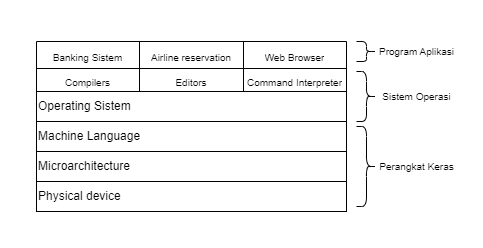
\includegraphics[width=1\textwidth]{asset/sistemoperasi.png}
		\caption{Sebuah komputer yang terdiri dari perangkat keras, sistem operasi, dan program aplikasi} 
		\label{fig:contoh_gambar}
	\end{figure}
    \item Referensi :
    \item Haryanto,E.V.(2012).\textit{Sistem Operasi Konsep dan Teori}.CV Andi Offset

\subsection{Process Description and Control}
Processes are a central concept in operating systems. This section covers:
\begin{itemize}
    \item Process states and state transitions
    \item Process control block (PCB)
    \item Context switching
\end{itemize}

\subsection{Scheduling Algorithms}
This section covers:
\begin{itemize}
    \item First-Come, First-Served (FCFS)
    \item Shortest Job Next (SJN)
    \item Round Robin (RR)
\end{itemize}
It explains how these algorithms are used to allocate CPU time to processes.

\subsection{Process Creation and Termination}
Details how processes are created and terminated by the operating system, including:
\begin{itemize}
    \item Process spawning
    \item Process termination conditions
\end{itemize}

\subsection{Introduction to Threads}
This section introduces the concept of threads and their relation to processes, covering:
\begin{itemize}
    \item Single-threaded vs. multi-threaded processes
    \item Benefits of multithreading
\end{itemize}

\begin{figure}[h]
    \centering
    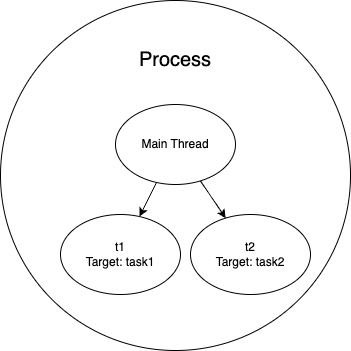
\includegraphics[width=0.5\textwidth]{/Users/khawaritzmi/Unhas/os_report_mid2024/b_class/asset/example.png}  % Sesuaikan nama file dan ukurannya
    \caption{Ini adalah gambar contoh dari multithreading.}
    \label{fig:contoh_gambar}
\end{figure}

Seperti yang terlihat pada Gambar \ref{fig:contoh_gambar}, inilah cara menambahkan gambar dengan keterangan.

\subsection{File Systems}
File systems provide a way for the operating system to store, retrieve, and manage data. This section explains:
\begin{itemize}
    \item File system structure
    \item File access methods
    \item Directory management
\end{itemize}

\subsection{Input and Output Management}
Input and output management is key for handling the interaction between the system and external devices. This section includes:
\begin{itemize}
    \item Device drivers
    \item I/O scheduling
\end{itemize}

\subsection{Deadlock Introduction and Prevention}
Explores the concept of deadlocks and methods for preventing them:
\begin{itemize}
    \item Deadlock conditions
    \item Deadlock prevention techniques
\end{itemize}

\subsection{User Interface Management}
This section discusses the role of the operating system in managing the user interface. Topics covered include:
\begin{itemize}
    \item Graphical User Interface (GUI)
    \item Command-Line Interface (CLI)
    \item Interaction between the user and the operating system
\end{itemize}

\subsection{Virtualization in Operating Systems}
Virtualization allows multiple operating systems to run concurrently on a single physical machine. This section explores:
\begin{itemize}
    \item Concept of virtualization
    \item Hypervisors and their types
    \item Benefits of virtualization in modern computing
\end{itemize}

\section{Assignments and Practical Work}
\subsection{Assignment 1: Process Scheduling}
Students were tasked with implementing various process scheduling algorithms (e.g., FCFS, SJN, and RR) and comparing their performance under different conditions.
\subsubsection{Group 1}
\begin{python}
    class Process:
    def __init__(self, pid, arrival_time, burst_time):
        self.pid = pid
        self.arrival_time = arrival_time
        self.burst_time = burst_time
        self.completion_time = 0
        self.turnaround_time = 0
        self.waiting_time = 0
\end{python}

\begin{table}[htbp] % Optional: For floating position
    \centering
    \begin{tabular}{|c|c|c|} % Defines number of columns and alignment (c = center, l = left, r = right). '|' creates vertical lines.
    \hline
    Header 1 & Header 2 & Header 3 \\ % Column headers
    \hline
    Row 1, Column 1 & Row 1, Column 2 & Row 1, Column 3 \\ % First row of data
    \hline
    Row 2, Column 1 & Row 2, Column 2 & Row 2, Column 3 \\ % Second row of data
    \hline
    \end{tabular}
    \caption{Your table caption} % Optional: For adding a caption
    \label{tab:your_label} % Optional: For cross-referencing the table
\end{table}
\subsubsection{Group 2}
\subsubsection{Group 3}
Implementasikan algoritma \textit{First-Come}, \textit{First-Served} (FCFS), \textit{Shortest Job Next} (SJN), dan \textit{Round Robin} (RR) untuk proses \textit{scheduling}. Bandingkan waktu eksekusi rata-rata \textit{(average waiting time)} dari ketiga algoritma tersebut dengan jumlah proses yang berbeda.
\begin{python}
    # FCFS Scheduling
def fcfs(processes):
    n = len(processes)
    wait_time = [0] * n
    for i in range(1, n):
        wait_time[i] = processes[i-1][1] + wait_time[i-1]
    avg_wait_time = sum(wait_time) / n
    return avg_wait_time

# SJN Scheduling
def sjn(processes):
    processes.sort(key=lambda x: x[1])  # Sort by burst time
    return fcfs(processes)

# RR Scheduling
def round_robin(processes, quantum):
    wait_time = [0] * len(processes)
    rem_burst_time = [p[1] for p in processes]
    t = 0
    while any(rem_burst_time):
        for i in range(len(processes)):
            if rem_burst_time[i] > 0:
                if rem_burst_time[i] > quantum:
                    t += quantum
                    rem_burst_time[i] -= quantum
                else:
                    t += rem_burst_time[i]
                    wait_time[i] = t - processes[i][1]
                    rem_burst_time[i] = 0
    avg_wait_time = sum(wait_time) / len(processes)
    return avg_wait_time

# Example usage
processes = [(1, 5), (2, 9), (3, 6)]  # (process_id, burst_time)
print("FCFS:", fcfs(processes))
print("SJN:", sjn(processes))
print("Round Robin:", round_robin(processes, 4))

\end{python}

\subsection{Assignment 2: Deadlock Handling}
In this assignment, students were asked to simulate different deadlock scenarios and explore various prevention methods.
\subsubsection{Group 1}
\subsubsection{Group 2}
\subsubsection{Group 3}
Simulasikan kondisi \textit{deadlock} pada sistem dengan 3 proses dan 2 \textit{resource}. Jelaskan dan implementasikan metode pencegahan \textit{deadlock} dengan metode \textit{"Banker’s Algorithm"}

\begin{python}
    # Banker's Algorithm
def is_safe(processes, available, max_demand, allocation):
    n = len(processes)
    m = len(available)
    need = [[max_demand[i][j] - allocation[i][j] for j in range(m)] for i in range(n)]
    finish = [False] * n
    safe_seq = []
    work = available[:]
    
    while len(safe_seq) < n:
        allocated = False
        for i in range(n):
            if not finish[i] and all(need[i][j] <= work[j] for j in range(m)):
                for j in range(m):
                    work[j] += allocation[i][j]
                safe_seq.append(i)
                finish[i] = True
                allocated = True
        if not allocated:
            return False, []
    
    return True, safe_seq

# Example Usage
processes = [0, 1, 2]
available = [3, 3]  # Available resources
max_demand = [[7, 5], [3, 2], [9, 0]]  # Maximum demand of each process
allocation = [[0, 1], [2, 0], [3, 3]]  # Allocated resources

safe, seq = is_safe(processes, available, max_demand, allocation)
if safe:
    print("Safe sequence exists:", seq)
else:
    print("System is in deadlock.")

\end{python}

\subsection{Assignment 3: Multithreading and Amdahl's Law}
This assignment involved designing a multithreading scenario to solve a computationally intensive problem. Students then applied **Amdahl's Law** to calculate the theoretical speedup of the program as the number of threads increased.

\subsection{Assignment 4: Simple Command-Line Interface (CLI) for User Interface Management}
Students were tasked with creating a simple **CLI** for user interface management. The CLI should support basic commands such as file manipulation (creating, listing, and deleting files), process management, and system status reporting.

\subsection{Assignment 5: File System Access}
In this assignment, students implemented file system access routines, including:
\begin{itemize}
    \item File creation and deletion
    \item Reading from and writing to files
    \item Navigating directories and managing file permissions
\end{itemize}

\section{Conclusion}
The first half of the course introduced core operating system concepts, including process management, scheduling, multithreading, and file system access. These topics provided a foundation for more advanced topics to be covered in the second half of the course.

\end{document}